\documentclass{beamer}
\usepackage[utf8]{inputenc}
\usepackage{graphicx}
\usetheme{default}
\usecolortheme{default}

\title[S01 Intro]{Section 01 : Introduction du cours}
\subtitle{GSF-3100 Marché des capitaux}
\author[SP. Boucher]{Simon-Pierre Boucher\inst{1}}
\institute[Université Laval]
{
  \inst{1}%
  Département de finance, assurance et immobilier\\
  Faculté des sciences de l'administration\\
  Université Laval}
\date[Automne 2021]{Automne 2021}

\begin{document}

\begin{frame}
  \titlepage
\end{frame}



\section{Coordonnées et disponibilités}
\begin{frame}{Coordonnées et disponibilités}{Introduction}
  \begin{block}{Simon-Pierre Boucher (Enseignant)}
\begin{itemize}
\item \textbf{Courriel:} simon-pierre.boucher.1@ulaval.ca
\item \textbf{Disponibilités:} Sur demande par courriel
\end{itemize}
\end{block}
  \begin{block}{Carlos Alberto Chaparro Sepulveda (Coordonnateur d'opérations)}
\begin{itemize}
\item \textbf{Courriel:} Carlos.Chaparro@fsa.ulaval.ca
\item \textbf{Disponibilités:} Sur demande par courriel pour vos questions en lien avec le travail de session
\end{itemize}
\end{block}
\end{frame}

\section{Contenu et activités}
\begin{frame}{Contenu et activités}{Introduction}
  \begin{block}{PARTIE I : CONCEPTS DE BASE DU MARCHÈ OBLIGATAIRE}
\begin{itemize}
\item \textbf{Section 01:} Introduction du cours
\item \textbf{Section 02:} Mathématiques financières des obligations
\item \textbf{Section 03:} Volatilité dans le marché obligataire
\item \textbf{Section 04:} Structure des taux d'intérêt
\end{itemize}
\end{block}
\end{frame}

\section{Contenu et activités}
\begin{frame}{Contenu et activités}{Introduction}
  \begin{block}{PARTIE II : LES MARCHÉS D'INTERMÉDIATION DE FONDS DE FINANCEMENT}
\begin{itemize}
\item \textbf{Section 05:} Marché monétaire
\item \textbf{Section 06:} Marché obligataire gouvernemental
\item \textbf{Section 07:} Marché des obligations corporatives
\item \textbf{Section 08:} Marché obligataire international
\end{itemize}
\end{block}
\end{frame}


\section{Contenu et activités}
\begin{frame}{Contenu et activités}{Introduction}
  \begin{block}{PARTIE III : LES MARCHÉS D'INTERMÉDIATION DE FONDS DE RISQUE}
\begin{itemize}
\item \textbf{Section 09:} Gestion de portefeuille obligataire
\item \textbf{Section 10:} Marché des titres adossés à des créances
\end{itemize}
\end{block}
\end{frame}


\section{Matériel didactique}
\begin{frame}{Matériel didactique}{Introduction}
  \begin{block}{Bond markets, analysis and strategies (9e édition)}
\begin{itemize}
\item Ce livre est recommandé, mais non obligatoire.
\item Auteur(s) : Fabozzi, Frank J.
\end{itemize}
\end{block}
\begin{center}
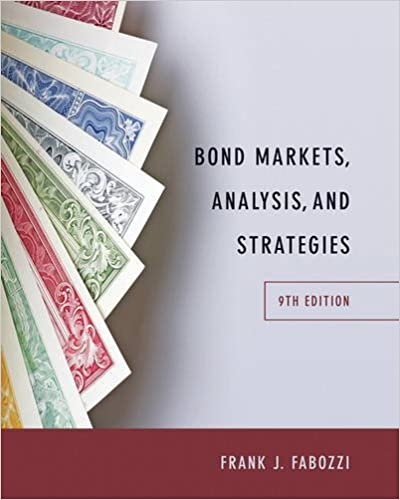
\includegraphics[scale=0.25]{BOOK}
\end{center}
\end{frame}



\section{Évaluations sommatives}
\begin{frame}{Évaluations sommatives}{Introduction}
  \begin{block}{Examen intra}
\begin{itemize}
\item \textbf{Période de disponibilité:} 	le 20 oct. 2021 de 18h30 à 21h20
\item \textbf{Durée:} 2 h 50 min
\item \textbf{Pondération:} 40\% de la note finale 
\item \textbf{Type:} Questions à choix multiples (50 questions)
\item \textbf{Déroulement:}  à distance 
\item \textbf{Matière à l'examen:} Section 01 à 08 inclusivement 
\end{itemize}
\end{block}
\end{frame}

\begin{frame}{Évaluations sommatives}{Introduction}
  \begin{block}{Examen final}
\begin{itemize}
\item \textbf{Période de disponibilité:} le 3 déc. 2021 de 18h30 à 21h20
\item \textbf{Durée:} 2 h 50 min
\item \textbf{Pondération:} 40\% de la note finale 
\item \textbf{Type:} Questions à choix multiples (50 questions)
\item \textbf{Déroulement:}  à distance 
\item \textbf{Matière à l'examen:} Section 09 à 10 inclusivement 
\end{itemize}
\end{block}
\end{frame}


\begin{frame}{Évaluations sommatives}{Introduction}
  \begin{block}{Travail de session}
\begin{itemize}
\item \textbf{Date de remise:} 30 nov. 2021 à 23h59
\item \textbf{Pondération:} 20\% de la note finale 
\item \textbf{Type:} Questions à choix multiples (50 questions)
\item \textbf{Équipe:} Quatre ou cinq étudiants
\item Le travail de session consiste à effectuer une étude approfondie de titres du marché des capitaux reliés au cours.
\end{itemize}
\end{block}
\end{frame}


\section{Objectif du cours}
\begin{frame}{GSF-3100: Marché des capitaux}{Introduction}
  \begin{block}{Objectif du cours:}
\begin{itemize}
\item Étudier les marchés financiers, ainsi que les actifs qui leur sont associés, dans leur rôle d’intermédiaire aux transferts de fonds entre les entités économiques déficitaires et les entités économiques excédentaires, et aux transferts de fonds de façon à redistribuer le risque. 
\item  Le cours se concentre sur les actifs reliés aux marchés des titres à revenu fixe ayant une échéance de moyenne ou longue durée.
\end{itemize}
  \end{block}
\end{frame}

\begin{frame}{GSF-3100: Marché des capitaux}{Introduction}
  \begin{block}{Plan de travail en trois parties:}
\begin{itemize}
\item Concepts de base du marché obligataire.
\item Les marchés d'intermédiation de fonds de financement.
\item Les marchés d’intermédiation de fonds de risque.
\end{itemize}
  \end{block}
  
  \begin{block}{Le but de cet introduction est:}
\begin{itemize}
\item De comprendre le concept de \textbf{marché d’intermédiation}.
\item De clarifier la différence entre les marchés de \textbf{fonds de financement} et ceux de \textbf{fonds de risque}.
\item D’introduire le marché obligataire.
\end{itemize}
  \end{block}
\end{frame}

\begin{frame}{Classes d'actifs}{Introduction}
\begin{itemize}
\item \textbf{Biens réels:}
\begin{itemize}
\item Ressources naturelles.
\item Capital physique.
\item Capital humain.
\item Capitale culturelle
\item Propriété intellectuelle
\end{itemize}
\item \textbf{Actifs financiers (appelés titres):}
\begin{itemize}
\item Argent
\item Dette
\item Capitaux propres
\item Dérivés
\item Combinaisons de ce qui précède
\end{itemize}
\end{itemize}
\end{frame}


\begin{frame}{Actifs financiers}{Introduction}
\begin{itemize}
\item \textbf{Argent:} un moyen d'échange (une créance papier soutenue par le gouvernement), est détenu pour permettre l'achèvement des transactions.
\item \textbf{Dette:} une créance sur un flux de paiement prédéterminé, généralement garanti par un ensemble d'actifs réels ou financiers.
\item \textbf{Capitaux propres:} créance résiduelle sur un ensemble d'actifs réels ou financiers (généralement d'une société) généralement associée au contrôle de la société.
\item \textbf{Dérivés:} le gain dépend de la valeur d'un autre actif (généralement financier).
\end{itemize}
\end{frame}

\section{Actif financier}
\begin{frame}{Actif financier}{Introduction}
\begin{itemize}
\item \textbf{Définition:} Promesse ou obligation d’honorer des engagements financiers.
\item \textbf{Valeur:} Valeur présente de ses flux monétaires.
\item  \textbf{Rôles:}
\begin{itemize}
\item Transfert de fonds entre les entités économiques déficitaires et les entités économiques excédentaires.  (\textbf{Fonds de financement.})
\vspace{0.5cm}
\item Transfert de fonds de façon à redistribuer le
risque.  (\textbf{Fonds de risque.})
\end{itemize}
\end{itemize}
\end{frame}

\begin{frame}{Le système financier}{Introduction}
\begin{itemize}
\item Désigne l'ensemble des institutions par lesquelles les actifs financiers sont créés et négociés.
\item \textbf{Objectifs:} qui permettent au système financier de créer de la richesse
\begin{itemize}
\item \textbf{Améliorer l'allocation du capital:} transférer le capital des épargnants (investisseurs) vers les utilisateurs de capital (généralement des sociétés).
\item \textbf{Améliorer l'allocation des risques:} transfert, partage et gestion des risques. Réduction de la prise de risque par le reconditionnement des risques.
\item \textbf{Timing de la consommation:} permettre aux investisseurs de lisser la consommation de manière intertemporelle.
\item \textbf{Séparation de la propriété et de la gestion}
\item \textbf{Discipliner les décisions d'investissement des entreprises.}
\end{itemize}
\end{itemize}
\end{frame}


\section{Intermédiation financière}
\begin{frame}{Intermédiation financière}{Introduction}
\begin{block}{Définition:}
Transformation d’actifs financiers sous forme de « nouveaux » actifs ou titres financiers préférables aux yeux des investisseurs.
\end{block}
\begin{block}{Exemples:}
\begin{itemize}
\item \textbf{Banque:} \\ Prêts, hypothèques $\rightarrow$ compte
d’épargne, certificat de dépôt.
\item \textbf{Compagnie d’assurance:} \\ Obligations, hypothèques $\rightarrow$ polices d’assurances
\end{itemize}
\end{block}

\end{frame}

\begin{frame}{Intermédiation financière}{Introduction}
\begin{block}{Types:}
\begin{itemize}
\item \textbf{Intermédiation de financement} (projets, maison, etc.).
\item \textbf{Intermédiation de risque} (liquidité, échéance, défaut, taux d’intérêt, diversification, etc.).
\end{itemize}
\end{block}
\begin{block}{Catégories d’intermédiaires financiers:}
\begin{itemize}
\item \textbf{Institutions financières} (ex: banque, compagnie
d’assurance, société de placements, etc.).
\item \textbf{Marchés financiers}.
\end{itemize}
\end{block}

\end{frame}

\section{Marché financier}
\begin{frame}{Marché financier}{Introduction}
\begin{itemize}
\item \textbf{Définition: Intermédiaire (lieu ou mécanisme) où s’échangent des actifs financiers.}
\item \textbf{Rôles secondaires:}
\begin{itemize}
\item Déterminer les prix.
\item Augmenter la liquidité.
\item Réduire les coûts de transaction.
\end{itemize}
\end{itemize}
\end{frame}


\begin{frame}{Marché financier}{Introduction}
\begin{block}{Marchés primaires vs marchés secondaires:}
\begin{enumerate}
\item \textbf{Marché primaire :} les nouvelles émissions d'un titre sont vendues aux premiers acheteurs.
\item \textbf{Marché secondaire :} les titres précédemment émis sont négociés sur un marché secondaire.
\end{enumerate}
\end{block}
\begin{block}{Marché d'échange vs marché de gré à gré:}
\begin{enumerate}
\item \textbf{Marché d'échange :} les acheteurs et les vendeurs de titres se rencontrent dans un endroit central pour effectuer des transactions.
\item \textbf{Marché de gré à gré :} Les courtiers à différents endroits sont prêts à acheter et à vendre des titres de \textbf{gré à gré} à toute personne qui accepte leurs prix.
\end{enumerate}
\end{block}
\end{frame}

\begin{frame}{Marché financier}{Introduction}
\begin{block}{Marchés monétaires vs. Marchés des capitaux:}
\begin{enumerate}
\item \textbf{Marché monétaire:} 
\begin{itemize}
\item instruments de dette à court terme
\item maturité $< 1$ an
\end{itemize}
\item \textbf{Marché des capitaux:}
\begin{itemize}
\item instruments de dette à long terme (revenu fixe)
\item maturité $> 1$ an
\end{itemize}
\end{enumerate}
\end{block}

\end{frame}




\section{Titre à revenu fixe}
\begin{frame}{Titre à revenu fixe}{Introduction}
\begin{block}{Définition:}
Instrument de dette qui requière à l’\textbf{émetteur/emprunteur} de repayer à l’\textbf{investisseur/prêteur} le montant emprunté plus les intérêts sur une période de temps spécifié et selon les termes du contrat.
\end{block}
\begin{block}{Acte de fiducie:}
Contrat entre l’\textbf{émetteur/emprunteur} et l’\textbf{investisseur/prêteur} qui spécifie les obligations de l’\textbf{émetteur/emprunteur}.
\end{block}
\end{frame}


\section{Titre à revenu fixe}
\begin{frame}{Titre à revenu fixe}{Introduction}
\begin{block}{Émetteurs:}
\begin{itemize}
\item Gouvernements
\item Sociétés
\item Banques commerciales 
\item États
\item Municipalités
\item SPV
\item Établissements étrangers
\end{itemize}
\end{block}
\end{frame}



\section{Titre à revenu fixe}
\begin{frame}{Titre à revenu fixe}{Introduction}
\begin{block}{Intermédiaires :}
\begin{itemize}
\item Principaux courtiers 
\item Banques d'investissement
\item Agences de notation 
\item Rehausseurs de crédit
\item Renforceurs de liquidité
\end{itemize}
\end{block}
\end{frame}


\section{Titre à revenu fixe}
\begin{frame}{Titre à revenu fixe}{Introduction}
\begin{block}{Investisseurs:}
\begin{itemize}
\item Gouvernements
\item Fonds de pension
\item Compagnies d'assurances 
\item Banques commerciales
\item Fonds communs de placement
\item Fonds spéculatifs
\item Établissements étrangers
\item Particuliers
\end{itemize}
\end{block}
\end{frame}


\begin{frame}{Titre à revenu fixe}{Introduction}
\begin{block}{Caractéristiques:}
\begin{itemize}
\item \textbf{Type d'émetteur :} Il existe trois émetteurs d'obligations.
\begin{itemize}
\item le gouvernement fédéral et ses agences
\item les gouvernements municipaux
\item les sociétés (nationales et étrangères).
\end{itemize}
\item \textbf{Échéance :} L'échéance d'une obligation fait référence à la date à laquelle la dette cessera d'exister, date à laquelle l'émetteur remboursera l'obligation en payant le principal.
\begin{itemize}
\item court terme : entre 1 et 5 ans 
\item moyen terme : entre 5 et 12 ans 
\item long terme : supérieur à 12 ans
\end{itemize}
\end{itemize}
\end{block}
\end{frame}

\begin{frame}{Titre à revenu fixe}{Introduction}
\begin{block}{Caractéristiques:}
\begin{itemize}
\item \textbf{Principal :} est le montant que l'émetteur s'engage à rembourser à l'obligataire à la date d'échéance. 
\begin{itemize}
\item Ce montant est également appelé valeur de remboursement, valeur à l'échéance et valeur nominale.
\end{itemize}
\item \textbf{Taux du coupon :} est le taux d'intérêt que l'émetteur s'engage à payer chaque année.
\begin{itemize}
\item Le montant annuel des intérêts versés aux propriétaires pendant la durée de l'obligation est appelé coupon.
\end{itemize}
\end{itemize}
\end{block}
\end{frame}


\begin{frame}{Titre à revenu fixe}{Introduction}
\begin{block}{Caractéristiques:}
\begin{itemize}
\item \textbf{Amortissement :}
Le remboursement du capital d'une émission obligataire peut nécessiter le remboursement du capital total soit à l'échéance, soit sur la durée de vie de l'obligation. 
\begin{itemize}
\item Dans le cas d'un remboursement sur sur la durée de vie de l'obligation, il existe un échéancier de remboursement du principal.
\end{itemize}
\item \textbf{Options intégrées :} Il est courant qu'une émission d'obligations inclue une disposition dans l'acte qui donne soit au détenteur de l'obligation et/ou à l'émetteur la possibilité de prendre des mesures contre l'autre partie.
\begin{itemize}
\item Le type d'option le plus courant incorporé dans une obligation est une clause d'achat.
\item Cette disposition confère à l'émetteur le droit d'annuler totalement ou partiellement la dette avant l'échéance prévue.
\end{itemize}
\end{itemize}
\end{block}
\end{frame}

\begin{frame}{Titre à revenu fixe}{Introduction}
\begin{block}{Description d'une émission obligataire}
\begin{itemize}
\item La plupart des titres sont identifiés par un numéro CUSIP à neuf caractères (lettres et chiffres).
\item CUSIP signifie \textbf{Committee on Uniform Security Identification Procedures}
\item Les six premiers caractères identifient l'émetteur : la société, l'organisme gouvernemental ou la municipalité.
\item Les trois derniers caractères sont utilisés pour catégoriser l'instrument émis sur le marché
\end{itemize}
\end{block}

\end{frame}


\begin{frame}{Titre à revenu fixe}{Introduction}
\begin{block}{Risques:}
\begin{itemize}
\item \textbf{Taux d’intérêt:} 
\begin{itemize}
\item Si un investisseur doit vendre une obligation avant la date d'échéance, une augmentation des taux d'intérêt entraînera la réalisation d'une perte en capital (comme la vente de l'obligation en dessous du prix d'achat).
\end{itemize}
\item \textbf{Réinvestissement:}
\begin{itemize}
\item Le risque de réinvestissement est le risque que le taux d'intérêt auquel les flux de trésorerie intermédiaires peuvent être réinvestis baisse.
\item Le risque de réinvestissement est plus important pour les périodes de détention plus longues, ainsi que pour les obligations avec des flux de trésorerie importants et précoces, telles que les obligations à coupon élevé.
\end{itemize}
\end{itemize}
\end{block}

\end{frame}



\begin{frame}{Titre à revenu fixe}{Introduction}
\begin{block}{Risques:}
\begin{itemize}

\item \textbf{Rachat:} 
\begin{itemize}
\item Le risque de Rachat est le risque que les investisseurs courent lorsqu'une obligation remboursable soit appelée lorsque les taux d'intérêt baissent.
\item De nombreuses obligations comportent une disposition qui permet à l'émetteur de se retirer ou de « racheter » tout ou partie de l'émission avant la date d'échéance.
\item L'émetteur conserve généralement ce droit afin d'avoir la possibilité de refinancer l'obligation à l'avenir si le taux d'intérêt du marché tombe en dessous du taux du coupon.
\end{itemize}
\item \textbf{Crédit et défaut:} 
\begin{itemize}
\item Le risque de crédit est le risque que l'émetteur d'une obligation ne respecte pas les conditions de l'obligation en ce qui concerne le paiement en temps voulu des intérêts et le remboursement du montant emprunté.
\item Cette forme de risque de crédit est appelée risque de défaut.
\end{itemize}
\end{itemize}
\end{block}

\end{frame}

\begin{frame}{Titre à revenu fixe}{Introduction}
\begin{block}{Risques:}
\begin{itemize}
\item \textbf{Inflation:} 
\begin{itemize}
\item Le risque d'inflation ou le risque de pouvoir d'achat découle de la variation de la valeur des flux de trésorerie d'un titre en raison de l'inflation, mesurée en termes de pouvoir d'achat.
\end{itemize}
\item \textbf{Taux de change:} 
\begin{itemize}
\item Une obligation non libellée en dollars (c'est-à-dire une obligation dont les paiements sont effectués dans une devise étrangère) a des flux de trésorerie inconnus en dollars américains
\item Les flux de trésorerie en dollars dépendent du taux de change au moment où les paiements sont reçus.
\item Le risque que le taux de change entraîne des flux de trésorerie plus faibles est appelé risque de change ou risque de change.
\end{itemize}
\end{itemize}
\end{block}

\end{frame}


\begin{frame}{Titre à revenu fixe}{Introduction}
\begin{block}{Risques:}
\begin{itemize}

\item \textbf{Liquidité:} 
\begin{itemize}
\item Le risque de liquidité ou de négociabilité dépend de la facilité avec laquelle une émission peut être vendue à ou près de sa valeur.
\item La principale mesure de la liquidité est la taille de l'écart entre le cours acheteur et le cours vendeur coté par un courtier.
\item Plus le spread du dealer est large, plus le risque de liquidité sera grand.
\end{itemize}
\item \textbf{Volatilité:}
\begin{itemize}
\item La valeur d'une option intégrée augmente lorsque la volatilité attendue des taux d'intérêt augmente.
\item Le risque
qu'un changement de volatilité affectera négativement le prix d'une obligation est appelé risque de volatilité.
\end{itemize}
\end{itemize}
\end{block}

\end{frame}

\begin{frame}{Banque du Canada}{Introduction}
\begin{itemize}
\item La \textbf{Banque du Canada} (en anglais : Bank of Canada) est la banque centrale du Canada. 

\item Elle est mise en place et régulée par la Loi sur la Banque du Canada.

\item En tant que banque centrale du pays, la \textbf{Banque du Canada} a quatre principaux domaines de responsabilité :

\begin{itemize}
\item Politique monétaire
\item Système financier
\item Monnaie
\item Gestion de fonds
\end{itemize}


\end{itemize}


\end{frame}



\begin{frame}{Banque du Canada}{Introduction}
\begin{block}{Politique monétaire}
\begin{itemize}
\item L'objectif de la \textbf{politique monétaire} est de préserver la valeur de la monnaie en maintenant l'inflation à un niveau bas, stable et prévisible
\item Le cadre de la \textbf{politique monétaire} du Canada se compose de deux éléments clés qui fonctionnent ensemble : 
\begin{itemize}
\item la cible de contrôle de l'inflation 
\item le taux de change flexible. 
\end{itemize}

\item Ce cadre aide à rendre les mesures de \textbf{politique monétaire} facilement compréhensibles et permet à la Banque de démontrer sa responsabilité envers les Canadiens.
\end{itemize}
\end{block}



\end{frame}

\begin{frame}{Banque du Canada}{Introduction}
\begin{block}{Politique monétaire}
\begin{itemize}
\item Pour atteindre l'objectif d'inflation, la Banque ajuste (\textbf{augmente ou diminue}) son taux directeur.
\item Si l'inflation est \textbf{supérieure} à la cible, la Banque peut relever le taux directeur.
\begin{itemize}
\item Cela encourage les institutions financières à augmenter les taux d'intérêt sur leurs prêts et hypothèques, décourageant les emprunts et les dépenses et atténuant ainsi la pression à la hausse sur les prix.
\end{itemize}
\item Si l'inflation est \textbf{inférieure} à la cible, la Banque peut abaisser le taux directeur.
\begin{itemize}
\item Cela encourage les institutions financières à baisser les taux d'intérêt sur leurs prêts et hypothèques et stimuler l'activité économique.
\end{itemize}
\end{itemize}
\end{block}



\end{frame}



\end{document}


\begin{frame}{Taux des obligations du Trésor américain}{Introduction}
\textbf{En rouge : Taux 1 ans}
\begin{center}
\includegraphics[scale=0.15]{1YEAR}
\end{center}

\end{frame}

\begin{frame}{Taux des obligations du Trésor américain}{Introduction}
\textbf{En bleu : Taux 5 ans}
\begin{center}
\includegraphics[scale=0.15]{5YEAR}
\end{center}

\end{frame}

\begin{frame}{Taux des obligations du Trésor américain}{Introduction}
\textbf{En vert : Taux 10 ans}
\begin{center}
\includegraphics[scale=0.15]{10YEAR}
\end{center}

\end{frame}

\begin{frame}{Taux des obligations du Trésor américain}{Introduction}
\textbf{En jaune : Taux 30 ans}
\begin{center}
\includegraphics[scale=0.15]{30YEAR}
\end{center}

\end{frame}


\begin{frame}{Courbes des rendements (USA)}{Introduction}
\textbf{En rouge : 2007}\\
\textbf{En bleu : 2019}\\
\textbf{En vert : 2021}

\begin{center}
\includegraphics[scale=0.14]{YC}
\end{center}

\end{frame}

\begin{frame}{Taux d'inflation (\%) : Canada}{Introduction}
\textbf{En rouge : fourchette cible de 1 à 3 \% à moyen terme}

\begin{center}
\includegraphics[scale=0.15]{INFLATION}
\end{center}

\end{frame}




